\title {\textbf{sorites update}}
\author {\textbf{erin}}
\date {\today}

\documentclass[10pt]{article}
\usepackage[numbers]{natbib}
\usepackage[colorlinks]{hyperref}
\usepackage {graphicx}
\usepackage {amsmath}
\usepackage {hyperref}
\usepackage {titling}
\usepackage[font = small]{caption}
\usepackage{gensymb}
\usepackage[margin = 0.5 in]{geometry}
\usepackage[toc,page]{appendix}

\begin{document}
\setlength{\droptitle}{-1.5cm}
\maketitle

\section{intro}
  We consider the following argument:
  
  \begin{itemize}
   \item[] \textbf{Premise 1:} The Sears Tower is tall.
   \item[] \textbf{Premise 2:} A building that is 1m shorter than a tall building is tall.
   \item[] \textbf{Conclusion:} Every building in Chicago is tall.
  \end{itemize}
  
  When people hear this argument, they tend to think that premise 1 (the ``concrete'' premise) and premise 2 (the ``inductive'' premise) are both clearly true, but that the conclusion -- which would naturally follow from the premises according to first order logic -- is clearly false.
  
  We explain people's reactions to these statements with a formal model of scalar adjective interpretation and show that their reactions are sensitive to the prior distribution on building heights and to the change in height $\epsilon$ given in the inductive premise (in this case, 1m).
  
\section{model}
  We use a model of scalar adjectives (e.g. ``tall'') in which a pragmatic listener must infer both the height that the speaker intended to communicate and also the threshold between ``tall'' and ``not tall'' that the speaker was using \cite{lassiter}. Because a speaker is likely to be communicating about things that are plausible in the world, but is unlikely to expend effort on uttering something uninformative, the pragmatic listener will infer that the threshold is high enough to be informative, but low enough for the communicated height to be plausible. This inference will depend on the speaker and listener's common ground on what plausible and likely heights are for a given category.
  
  \subsection{initial simulations of adjective model and effects of parameters}
    We can look at this model's inferences about the threshold $\theta$ and the degree $x$ (in the previous example, height) when the prior distribution is roughly gaussian with mean 50 and standard deviation 20. Different rationality parameters $\alpha$ and different costs $C$ for the scalar adjective utterance (e.g. ``tall'') result in different posterior distributions on $\theta$ and $x$.
    
    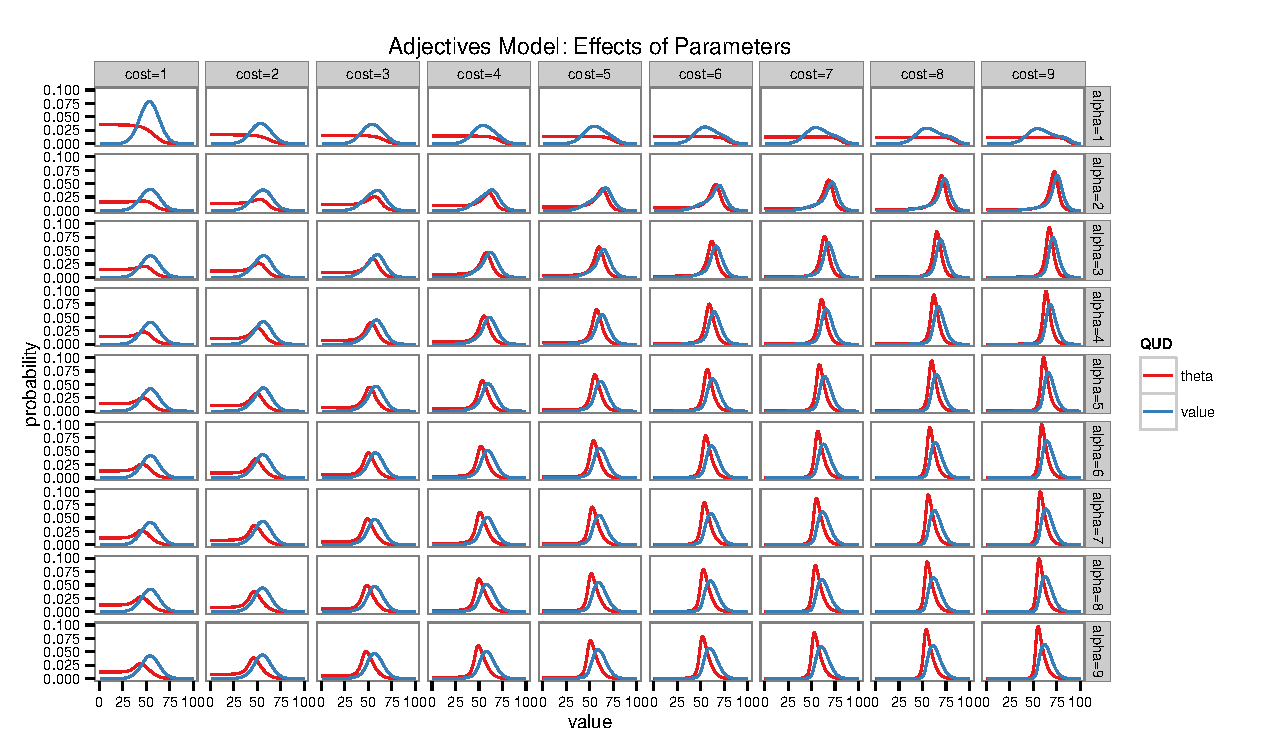
\includegraphics[width=0.9\textwidth]{toy_parameter_search.pdf}
    
    As cost increases, the model infers the threshold variable $\theta$ and the degree $x$ to be higher. As rationality parameter $\alpha$ increases, the model's posterior becomes peakier, moving probability mass away from unlikely values and towards higher probability ones.
    
%     The simulations above are with no alternative utterances. We can run the model with an additional possible utterance for the speaker that means the opposite of ``tall'' and has its own threshold variable.
%     
%     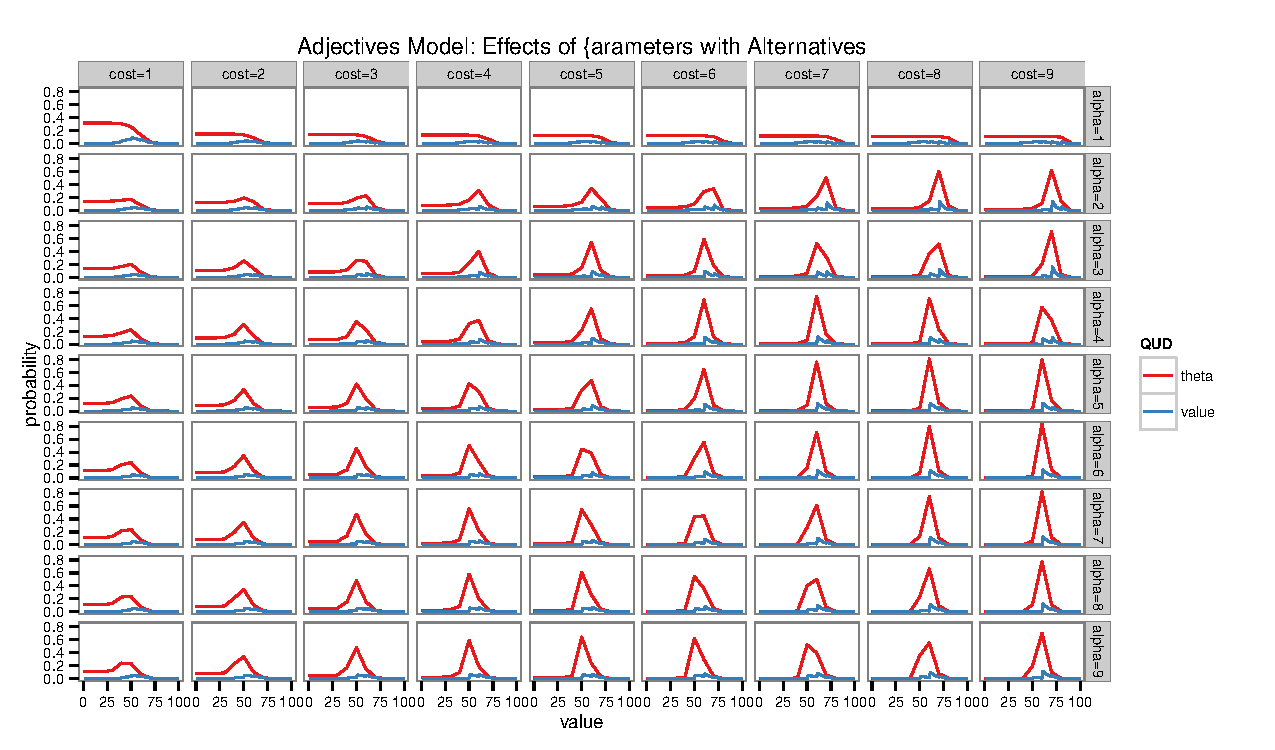
\includegraphics[width=0.9\textwidth]{toy_parameter_search_alternatives.pdf}
    
  \subsection{applying adjective model to sorites}
    In order to interpret the sorites argument, our model first infers a value of the threshold variable $\theta$ and the degree $x$, conditioned on a speaker saying the scalar adjective. The model then evaluates the following expressions:
        
    \begin{itemize}
    \item[] \textbf{Premise 1:} $height(\mbox{Sears Tower}) > \theta_{tall}$
    \item[] \textbf{Premise 2:} $height(x) - 1 > \theta_{tall}$
    \item[] \textbf{Conclusion:} $\forall y \in \{ \mbox{buildings in Chicago} \}, \ height(y) > \theta_{tall}$
    \end{itemize}
    
    The expressions for premises 1 and 2 are likely (but not guaranteed) to be true. The expression for the conclusion, however, is unlikely to be true. This interpretation of the sorites argument predicts that as the amount of change in height $\epsilon$ (in this case 1m) changes, endorsement of the inductive premise will change, since the probability of $height(x) - \epsilon > \theta_{tall}$ becomes lower as $\epsilon$ increases. We test this prediction, as well as sensitivity to the prior distribution.
    
\section{prior elicitation(s)}
  In order to compare model predictions to humans, we chose to look at prices of everyday items. This is a domain where humans have relatively consistent prior knowledge and where the scale is representable as numeric quantities.
  
  We first measured people's prior distributions over prices in a series of experiments.

  \subsection{basic setup}
    We gave people a number of bins, each bin representing a range of prices, and asked how likely an object would be to cost a price within each range. Within each of the three versions of this kind of prior elicitation experiment, we gave participants the same bins for each object. There were many bins, so there were multiple rows of sliders that participants had to mark.
  
    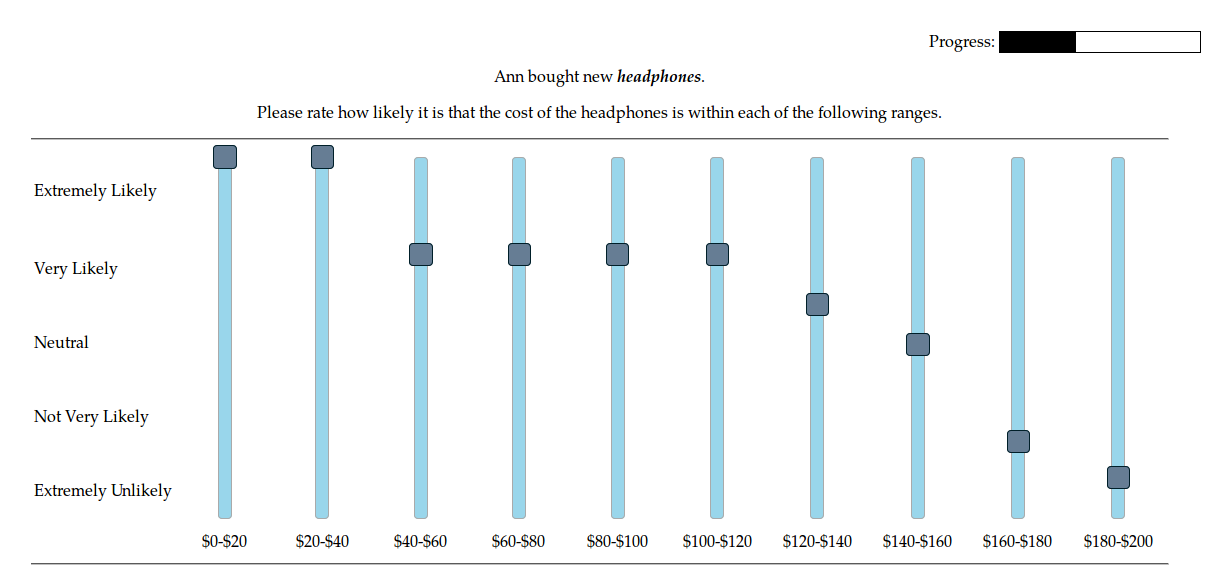
\includegraphics[width=0.6\textwidth]{screenshot1.png}
    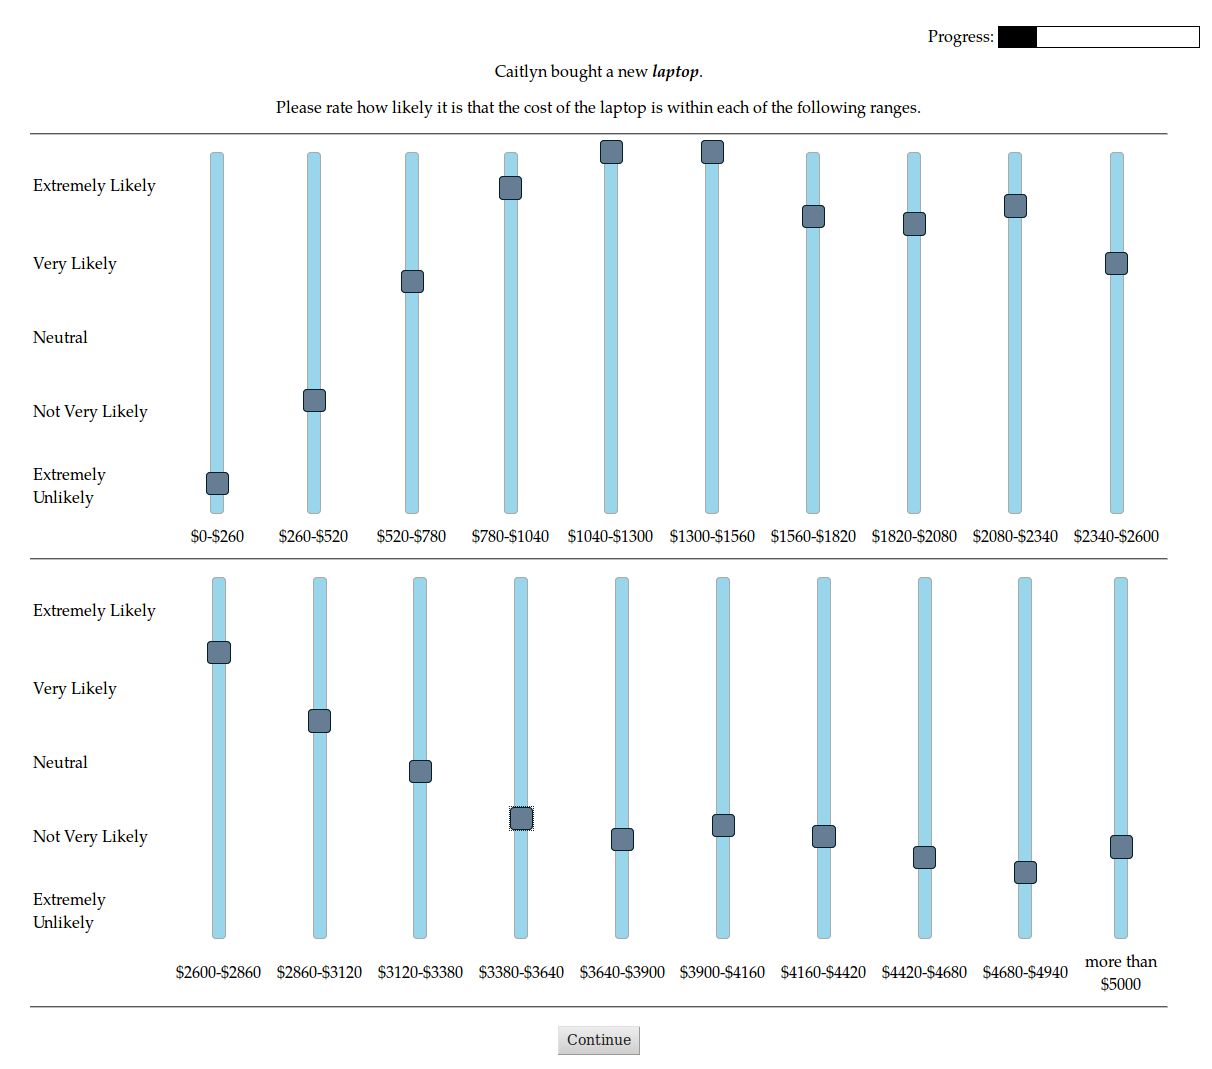
\includegraphics[width=0.3\textwidth]{screenshot2.png}
    
  \subsection{results}
    We ran three different versions of these experiments, each with different ranges and bin widths for the different items. We found similar responses across all of the experiments. Version A (10 participants, 1 outlier excluded) had 40 bins for each of the 5 objects, Version B (10 participants) had more bins (the number varied by object), and Version C (36 participants) had fewer objects in the experiment design. Because we had the best coverage of objects and ranges in Version B, and because its results are similar to those found in other versions, I use the prior elicitation data from Version B in the model simulations that follow.
    
    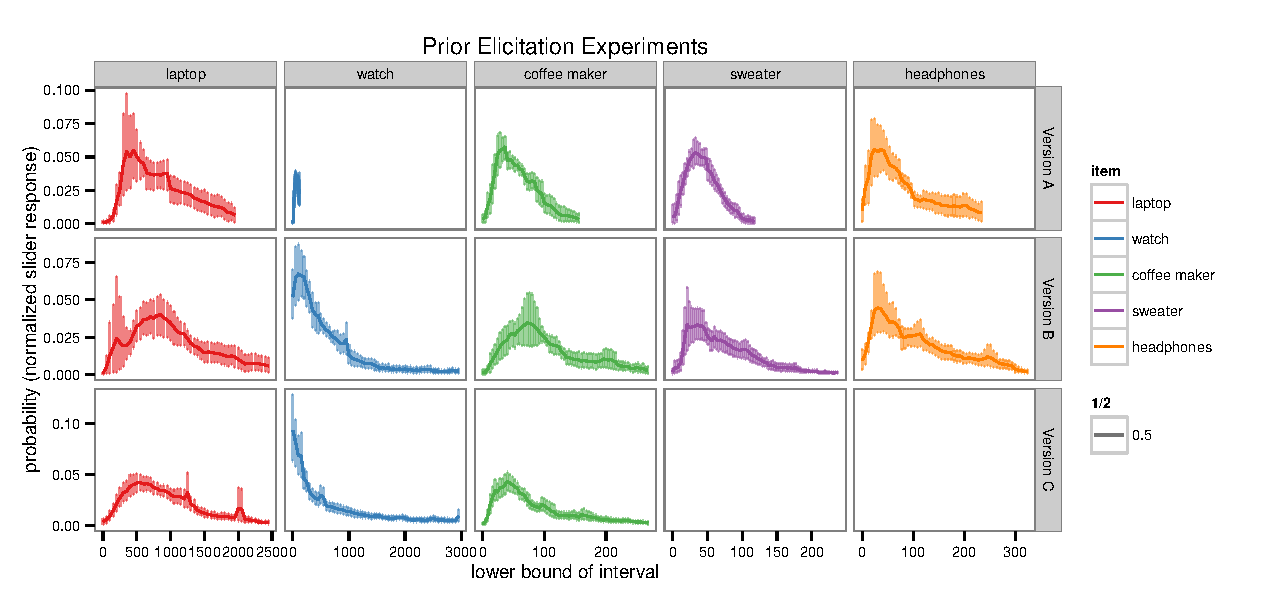
\includegraphics[width=0.8\textwidth]{all_bins_priors.pdf}
    
%   \subsection{scraped priors}
%     In addition to the bins prior elicitation experiments, we also scraped prices from Amazon and Ebay. In previous analyses, I used the prices scraped from Ebay. These priors are similar, but overall much peakier than the distributions elicited from people. However, I don't know how to get the density with reasonable bins yet, so ignore this.
%     
%     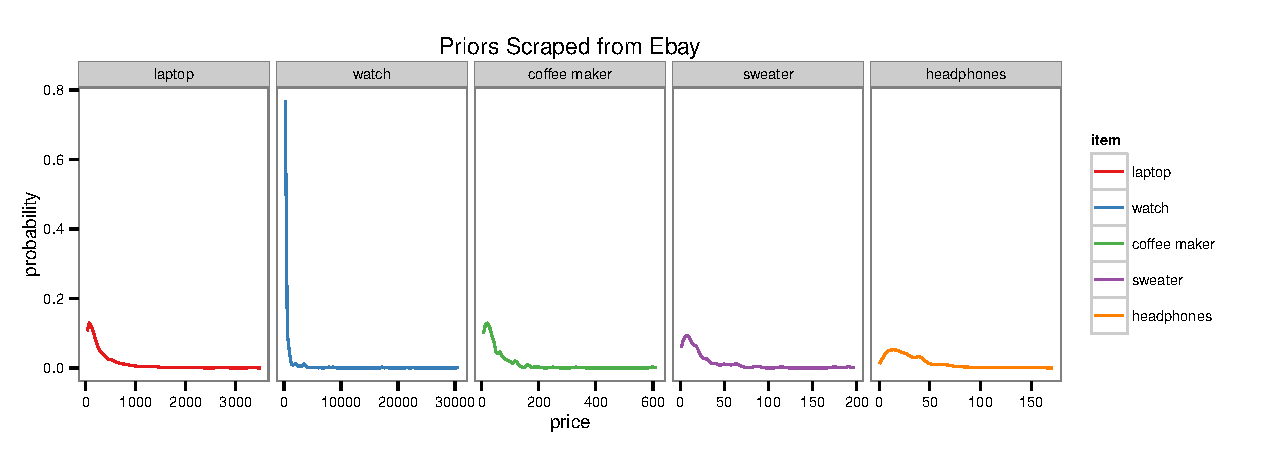
\includegraphics[width=0.8\textwidth]{ebay_priors.pdf}
%     
% %   \subsection{discussion}
% %     \subsubsection{discontinuity at linebreak}
% %       %unsmoothed graphs
% %     \subsubsection{other possible sampling strategies?}
% %       \paragraph{the full bayesian thing}
% %       \paragraph{individual bins}
% %       \paragraph{cdf}
% 
\section{simulations}

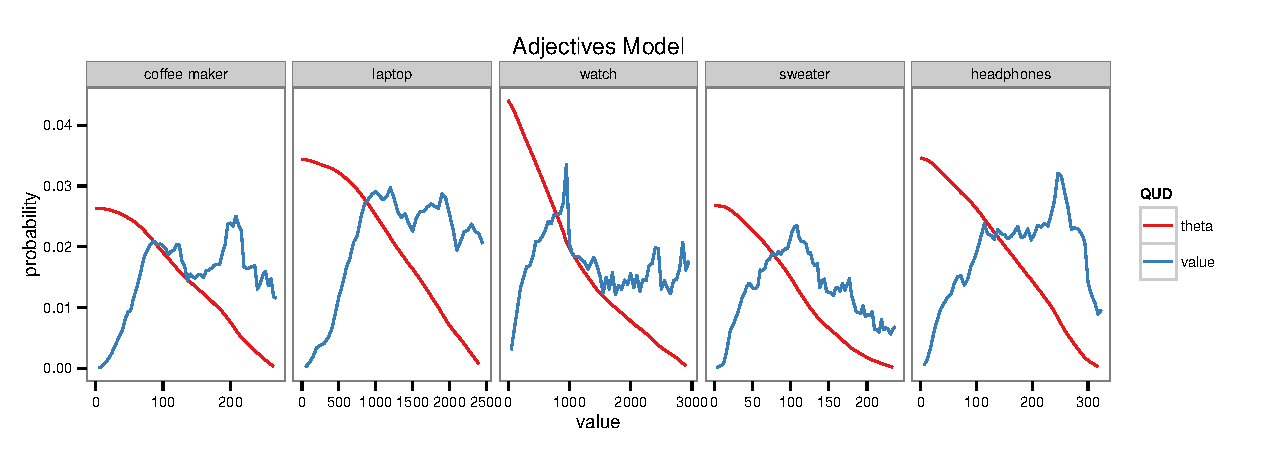
\includegraphics[width=0.8\textwidth]{adjective.pdf}

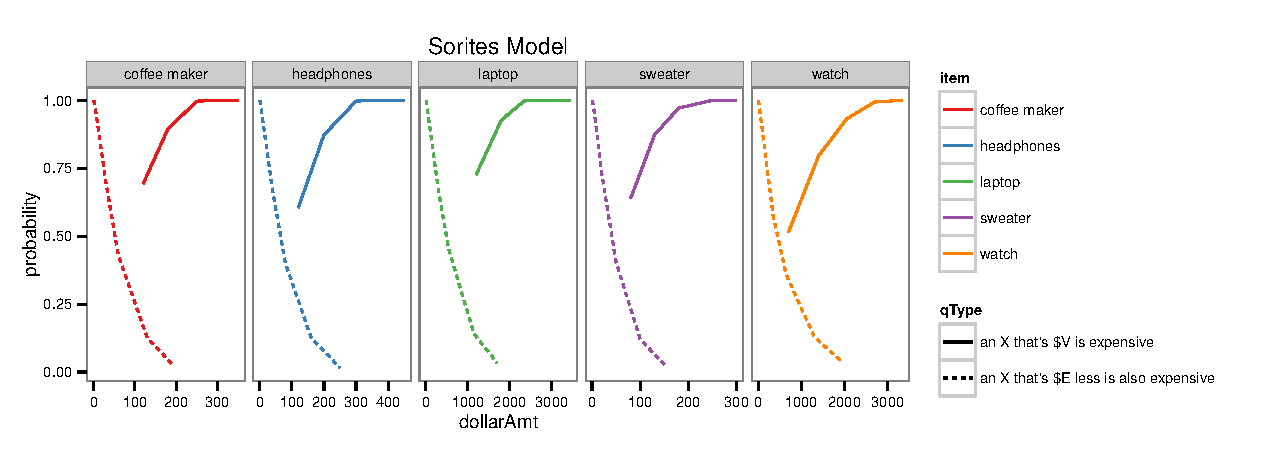
\includegraphics[width=0.8\textwidth]{sorites_model.pdf}

\section{experiment}

\section{comparison}
% 
% \section{sorites experiment}
% 
% 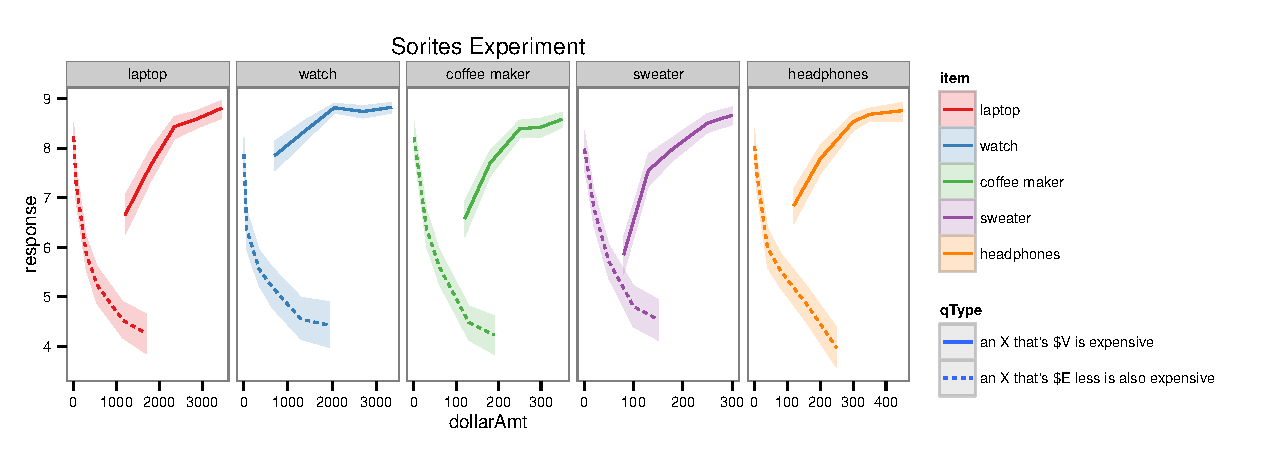
\includegraphics[width=0.8\textwidth]{sorites-experiment.pdf}
% 
% 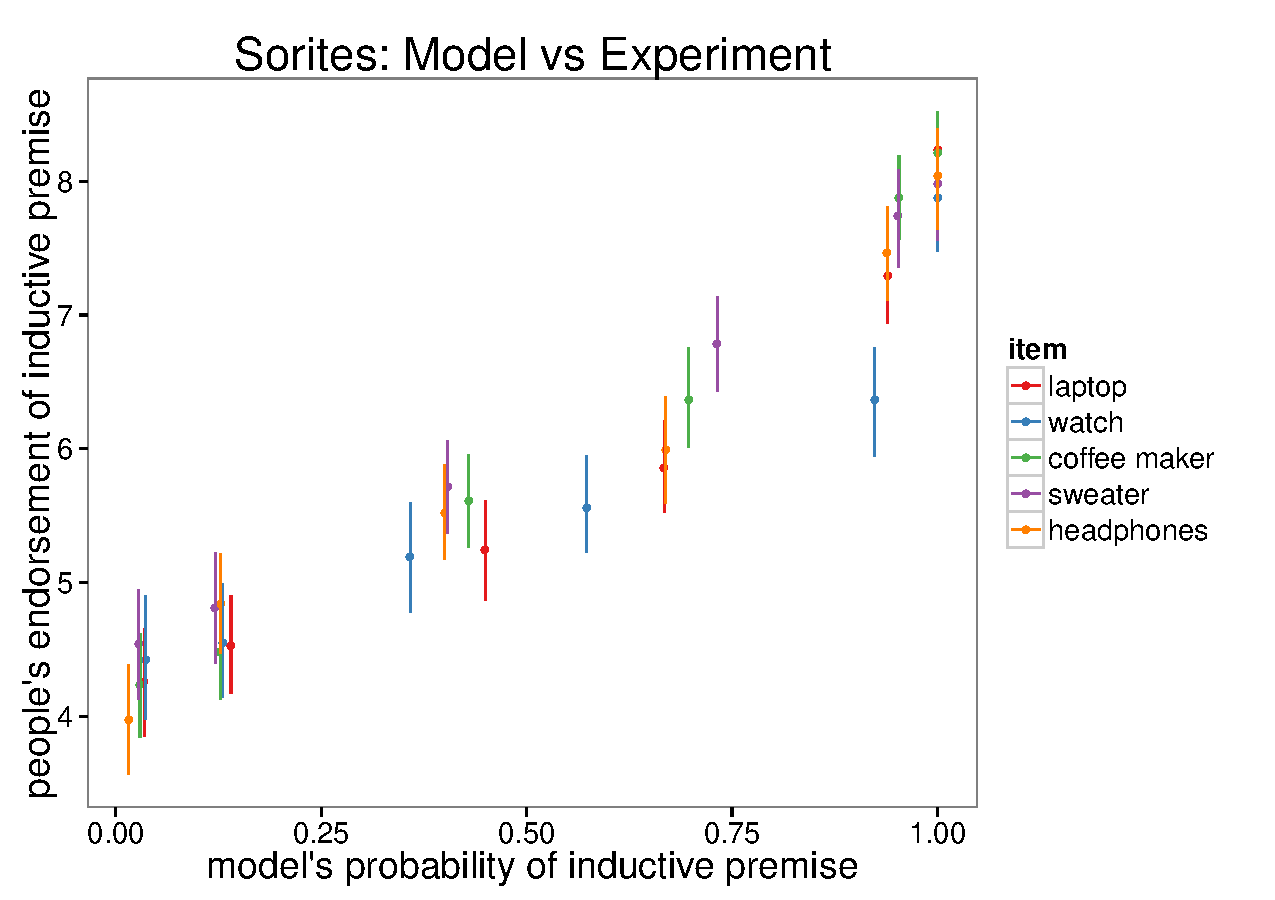
\includegraphics[width=0.5\textwidth]{sorites-model-vs-people.pdf}
% 
% Pearson's product-moment correlation: 0.966776.

% \section{discussion}

\end {document}